\documentclass{article}
\usepackage{mathrsfs}
\usepackage{amsmath}
\usepackage{amssymb}
\usepackage{braket}
\usepackage[normalem]{ulem} % for strikeout line
\usepackage{graphicx}
\graphicspath{ {./images/} }
% \usepackage{epstopdf}

%-------------------------------------------------------%
\newcounter{pcounter}                                   %
\newenvironment{problem}                                %
{                                                       %
    \stepcounter{pcounter}                              %
    \textbf{\arabic{pcounter}.}                         %
}{}                                                     %
\newenvironment{solution}                               %
{\textbf{Solution:} \\}{$\blacksquare$\newline}         %
%-------------------------------------------------------%
\newcommand{\tab}{\ \ \ \ }                             %
\newcommand{\leadto}{\Rightarrow}                       %
\newcommand{\domR}{\mathcal{R}}                         %
\newcommand{\domS}{\mathbb{S}}                          %
\newcommand{\Gaussian}{\mathcal{N}}                     %
\newcommand{\IdenMat}{\textit{I}}                       %
\newcommand{\abss}[1]{\| #1 \|}                         %
\newcommand{\tr}[1]{\textbf{tr}(#1)}                    %
\newcommand{\vecOne}{\textbf{1}}                        %
%-------------------------------------------------------%

\begin{document}
    %------------------- The Title -------------------%
    \parindent 0in
    \parskip 1em
    \title{COMP9501 Assignment 1 Solution Sheet}
    \author{HONG Yuncong, 3030058647}
    \maketitle

    %=================== Problem 1 ===================%
    \begin{problem}
        We have two random variables $X$ and $Y$.
        X follows the standard Gaussian distribution:
        $$
        p(x) = \Gaussian(x | 0, \IdenMat),
        $$
        where $x$ is a $m$-dim vector, and $\IdenMat$ is the identity matrix. $Y|X$ also follows a Gaussian distribution:
        $$
        p(y|x) = \Gaussian(y | \mu+\Lambda x, \Psi),
        $$
        where $y$ is a $n$-dim vector, $\Lambda \in \domR^{n \times m}$ is called the factor loading matrix, $\mu$ is a constant vector, and $\Psi$ is a \textbf{diagonal covariance matrix}.

        (1) [Joint Distribution] Prove that the joint distribution of $(X, Y)$ is
        $$
        p(
            \begin{pmatrix}
                x \\ y
            \end{pmatrix}
        ) = 
        \Gaussian(
            \begin{pmatrix}
                x \\ y
            \end{pmatrix}
            |
            \begin{pmatrix}
                0 \\ \mu
            \end{pmatrix}
            ,
            \begin{pmatrix}
                \IdenMat & \Lambda^T \\
                \Lambda & \Lambda \Lambda^T + \Psi
            \end{pmatrix}
        )
        $$

        (2) [Posterior Distribution] Prove that the posterior distribution $X|Y$ is $p(x|y) = \Gaussian(x|\mu_{x|y}, \Sigma_{x|y})$, where
        \begin{gather*}
            \mu_{x|y} = \Sigma \Lambda^T \Psi^{-1} (Y - \mu) \\
            \Sigma_{x|y} = (\IdenMat + \Lambda^T \Psi^{-1} \Lambda)^{-1}
        \end{gather*}

        (3) [Incomplete log likelihood] The incomplete log likelihood is defined according to the marginal density of $Y$:
        $$
        l(\theta, \mathcal{D}) = log \prod\limits_{i=1}^{n} p(y_i)
        $$
        \tab a) Please compute the incomplete log likelihood, which should involve $\Lambda, \Psi$, and adata covariance matrix 
        $S=\sum_{i=1}^n (y_i - \mu)(y_i - \mu)^T$
        
        \tab b) Try to compute the MLE estimate for $\theta = (\Lambda, \Psi)$ and explain what is the main difficulty that prevents you from getting the result.

        (4) [Complete log likelihood] The complete log likelihood is defined as 
        $$
        l_c(\theta, \mathcal{D}) = log \prod\limits_{i=1}^{n} p(x_i, y_i)
        $$
        \tab a) Please compute the complete log likelihood, which should involve $\Lambda, \Psi$, and adata covariance matrix 
        $S=\frac{1}{n} \sum_{i=1}^n (y_i - \Lambda x_i)(y_i - \Lambda x_i)^T$

        \tab b) Try to compute the MLE estimate for $\theta = (\Lambda, \Psi)$ and explain why it is simpler that 1.3(b).
    \end{problem}

    \begin{solution}
        {[}The solution in (1) and (2) uses the "Useful Porperties of Gaussian" on the slides. The proof processes of the two should resembles in the same form and regardless of the order of the two random variables $X$ and $Y$; so the proof process is obsoleted{]}

        (1) Assume that the joint distribution of $(X, Y)$ is
        $$
        p(\begin{pmatrix}
            x \\ y
        \end{pmatrix}) = 
        \Gaussian(
            \begin{pmatrix}
                x \\ y
            \end{pmatrix}
            | 
            \begin{pmatrix}
                \mu_x \\ \mu_y
            \end{pmatrix}, 
            \begin{pmatrix}
                \Sigma_{x} & \Sigma_{xy} \\
                \Sigma_{yx} & \Sigma_{y}
            \end{pmatrix}
        )
        $$
        As marginal distribution of $x$ is $p(x) = \Gaussian(x | 0, \IdenMat)$, we know that: 
        \begin{align*}
            & \mu_x = 0 \\
            & \Sigma_{x} = \IdenMat
        \end{align*}
        and by the "known useful properties of Gaussian" on the slides, we know that:
        \begin{align*}
            \mu_{y|x} = \mu_y + \Sigma_{yx} \Sigma_{x}^{-1}(x - \mu_x) \\
            \Sigma_{y|x} = \Sigma_{y} - \Sigma_{yx} \Sigma_{x}^{-1} \Sigma_{xy}
        \end{align*}
        As $p(y|x) = \Gaussian(y | \mu+\Lambda x, \Psi)$, we know that:
        \begin{align*}
            \mu_y &= \mu \\
            \Lambda = \Sigma_{yx} 
                &\leadto \Sigma_{yx}=\Sigma_{xy}^T=\Lambda\\
            \Psi = \Sigma_{y} - \Sigma_{yx} \Sigma_{xy}
                &\leadto \Sigma_{y} = \Psi + \Sigma_{yx} \Sigma_{xy}
        \end{align*}
        And with all the information above we could have:
        $$
        p(
            \begin{pmatrix}
                x \\ y
            \end{pmatrix}
        ) = 
        \Gaussian(
            \begin{pmatrix}
                x \\ y
            \end{pmatrix}
            |
            \begin{pmatrix}
                0 \\ \mu
            \end{pmatrix}
            ,
            \begin{pmatrix}
                \IdenMat & \Lambda^T \\
                \Lambda & \Lambda \Lambda^T + \Psi
            \end{pmatrix}
        )
        $$

        (2) for $p(x|y)$: similarly, we use the properties mentioned in (1) and we have:
        \begin{align*}
            \mu_{x|y} &= \Sigma{x|y}(\Lambda_{x}\mu_x-\Lambda_{xy}(y-\mu_y)) \\
            &= \Sigma_{x|y}(-\Lambda_{xy})(y-\mu) \\
            &= \Sigma_{x|y}[I^{-1} \Lambda^T (\Lambda \Lambda^T+\Psi-\Lambda I^{-1} \Lambda^T)^{-1}](y-\mu) \\
            &= \Sigma_{x|y} \Lambda^T \Psi^{-1}(y-\mu)
            \\
            \Sigma_{x|y} &= \Sigma_x - \Sigma_{xy} \Sigma_y^{-1} \Sigma_{yx} \\
            &= I - \Lambda^T (\Lambda \Lambda^T + \Psi)^{-1} \Lambda \\
            &= (I + \Lambda^T \Psi^{-1} \Lambda)^{-1}
        \end{align*}

        (3) \\
        a) As we know that $p(y) = \Gaussian(y|\mu, \Psi+\Lambda \Lambda^T)$,
        \begin{align*}
            l(\theta, \mathcal{D}) &= log \prod_{i=1}^{n}{p(y_i)} \\
            &= log \prod_{i=1}^{n} |2 \pi \Sigma_y|^{-1/2} exp\{-1/2 (y_i-\mu)^T \Sigma_y^{-1} (y_i-\mu)\} \\
            &= -\frac{1}{2} \sum_{i=1}^{n} log(|2 \pi \Sigma_y|)
               -\frac{1}{2} \sum_{i=1}^{n}{(y_i-\mu)^T \Sigma_y^{-1} (y_i-\mu)} \\
            &= -\frac{1}{2} \sum_{i=1}^{n} \{log(|2 \pi \Sigma_y|) + (y_i-\mu)^T \Sigma_y^{-1} (y_i-\mu)\} \\
            &= -\frac{1}{2} \{
                n \cdot log|2\pi(\Psi+\Lambda \Lambda^T)| + tr[(\Psi+\Lambda \Lambda^T)^{-1} S]
            \}
        \end{align*}
        \\
        b) The MLE estimate may hard to compute cause $\Lambda \Lambda^T + \Psi^{-1}$ is highly coupled and could not be calculated;

        (4) \\
        a)
        \begin{align*}
            l_c(\theta, \mathcal{D}) &= log \prod_{i=1}^{n}{p(x_i, y_i)} \\
            &= log \prod_{i=1}^{n} \{p(x_i) \cdot p(y_i|x_i)\} \\
            &= -\frac{1}{2}\{2n\pi \cdot log|I| + \sum_{k=1}^{n} x_i^T x_i\}
               -\frac{1}{2}\{2n\pi \cdot log|\Psi| + \sum_{i=1}^{n}(y_i-\mu-\Lambda x_i)^T \Psi^{-1} (y_i-\mu-\Lambda x_i)\} \\
            &= -\frac{1}{2}\{n log|2 \pi \Psi| + \sum_{i=1}^{n}{x_i^T x_i} + n \cdot tr[S \Psi^{-1}]\}
        \end{align*} \\
        b) \\
        \begin{align*}
            & \frac{\partial l_{\theta, \mathcal{D}}}{\partial \Psi} = 0 \\
            \leadto &
                \Psi^{-1} - S \Psi^{-1} \Psi^{-1} = 0 \\
            \leadto &
                \Psi = S
            \\
            \\
            & \frac{\partial l_{\theta, \mathcal{D}}}{\partial \Lambda} = 0 \\
            \leadto &
                -2 \Psi^{-1} \sum_{i=1}^{n}{(y_i - \Lambda x_i)x_i^T} = 0 \\
            \leadto &
                \sum_{i=1}^{n}(y_i x_i^T) = \Lambda \sum_{i=1}^{n}(x_i x_i^T) \\
            \leadto &
                \Lambda = (\sum_{i=1}^{n}y_i x_i^T) \cdot (\sum_{i=1}^{n}x_i x_i^T)^{-1}
        \end{align*}      

        Reference:\\
        \text{[1] https://www.cs.cmu.edu/~epxing/Class/10708-14/scribe\_notes/scribe\_note\_lecture11.pdf}
        \text{[2] https://www.ics.uci.edu/~welling/teaching/KernelsICS273B/MatrixCookBook.pdf}
    \end{solution}

    %=================== Problem 2 ===================%
    \begin{problem}
        Let $X$ be an i.i.d collection of random variables from a Poisson distribution with parameter $\lambda$, $X \sim Poisson(\lambda)$, where $\lambda > 0$

        (1) [Basic Concepts and Properties]

        \tab a) Write out the exponential family form of X
        
        \tab b) Determine the sufficient statistics of $X$ for the Poisson distribution, i.e. $T(x)$
        
        \tab c) Write out the log-partition function of $X$, i.e. $A(\eta)$
        
        \tab d) Determine the response function (i.e., the inverse of the link function)
        
        \tab e) Determine $E[X]$ and $Var[X]$ using the log-partition function
        
        \tab f) Write out the MLE of $\lambda$ for data $X=\{x_1, \dots, x_n\}$
        
        \tab g) Let $\lambda \sim Gamma(\alpha, \beta)$, where $\alpha, \beta > 0$. The Gamma distribution is conjugate to the Poisson distribution,$ Gamma(\alpha, \beta) \propto x^{\alpha - 1} / e^{\beta x}$. Write out the MAP of $\lambda$ given $X=\{x_1, \dots, x_n\}$ .

        (2) [MLE and MAP simulation] \\
        For this problem, \textbf{please use the data labled HW1.txt}. This file contains a column array of 10,000 integer values, where each value represents the number of customers that entered a 24-hour laundromat in one hour intervals, over 10,000 hours.
        Let $X = \{x_1, \dots, x_t, \dots, x_n\}$ represents this column array, where $x_t$ is the number of customers that entered during the $t$-th hour. The hourly arrival of customers can be modeled as a collection of i.i.d. random variables drawn from a Poisson distribution $X \sim Poisson(\lambda)$, where $\lambda$ is the hourly arrival rate.
        
        \tab a) Plot a histogram of $X$ using 25 bins.
        
        \tab b) Using your answer from 2.1, compute the MLE of $\lambda$ for the observed data $X$ 

        For parts c) - e) model the hourly arrival rate $\lambda$ as having a Gamma distribution $\lambda \sim Gamma(\alpha, \beta)$, where $\alpha, \beta > 0$. Use your answer from 2.1(g) to:
        
        \tab c) Compute the MAP of $\lambda$ given $X$ for $\alpha = 1$ and $\beta = 1$
        
        \tab d) Compute the MAP of $\lambda$ given $X$ for $\alpha = 100$ and $\beta = 1$
        
        \tab e) Compute the MAP of $\lambda$ given $X$ for $\alpha = 10$ and $\beta = 1$

        \tab f) which approximation to $\lambda$ in b)-e) do you think is the best? How much does the prior distribution, and parameterizations of the prior in particular, impact the MAP estimates of $\lambda$? (One or Two sentences)
    \end{problem}

    \begin{solution}
        (1) [Basic Concepts and Properties]

        (a) \\
        As we know that for 1-D Poisson distribution, $p(x | \lambda) = e^{-\lambda} \frac{\lambda^x}{x!}$; then for i.i.d collection Poisson distribution r.v. collection X,
        \begin{align*}
            p(X | \lambda) &= \prod\limits_{i=1}^{N} e^{-\lambda} \frac{\lambda^{x_i}}{x_i!} \\
            &= (\prod\limits_{i=1}^{N}{\frac{1}{x_i!}}) \cdot
               exp\{ log{\lambda}\sum\limits_{i=1}^{N}{x_i} - \sum\limits_{i=1}^{N}{\lambda} \} \\
        \end{align*}
        where:
        \begin{align*}
            & h(x) = \prod\limits_{i=1}^{N}{\frac{1}{x_i!}} \\
            & T(x) = \sum\limits_{i=1}^{N}{x_i}\\
            & \eta = log{\lambda}\\
            & A(\eta) = \sum\limits_{i=1}^{N}{\lambda} = \sum\limits_{i=1}^{N}{e^{\eta}} \\
            & \text{($N$ is the number of the collection of random variables)}
        \end{align*}

        (b) sufficient statistics of $X$: $T(x) = \sum\limits_{i=1}^{N}{x_i}$

        (c) log-partition function of $X$: $A(\eta) = \sum\limits_{i=1}^{N}{\lambda} = \sum\limits_{i=1}^{N}{e^{\eta}}$

        (d) response function
        $$
            \mu = \frac{\partial A(\eta)}{\partial \eta}
            = \sum\limits_{i=1}^{N}{e^{\eta}}
        $$

        (e)
        As we know that:
        \begin{align*}
            E[T(X)|\eta] &= \frac{\partial A(\eta)}{\partial \eta}
            = \sum\limits_{i=1}^{N}{e^{\eta}}
            \\
            Var[T(x)^2|\eta] &= \frac{\partial^2 A(\eta)}{\partial \eta^2}
            = \sum\limits_{i=1}^{N}{e^{\eta}}
            \\
            T(x) &= \sum_{i=1}^{N}{x_i}
        \end{align*}
        As the components of $X$ are i.i.d, we could easily obtain that:
        \begin{align*}
            E[X|\eta] &= (E[X_1], \dots, E[X_n])^T \\
            &= (E[T(X)]/N, \dots, E{T(X)}/N)\\
            &= (e^\eta, \dots, e^\eta)^T
            \\
            Var(X|\eta) &= E[(X-E[X])(X-E[X])^T] \\
            &= \begin{pmatrix}
                Var[X_1] & 0 & \dots & 0 \\
                0 & Var[X_2] & \dots & 0 \\
                \vdots & \vdots & \ddots & \vdots \\
                0 & 0 & \dots & Var[X_N]
            \end{pmatrix} \\
            &= \begin{pmatrix}
                e^{\eta} & 0 & \dots & 0 \\
                0 & e^{\eta} & \dots & 0 \\
                \vdots & \vdots & \ddots & \vdots \\
                0 & 0 & \dots & e^{\eta}
            \end{pmatrix}
        \end{align*}

        (f) As data $X=\{x_1, \dots, x_n\}$ are fed to i.i.d random variables respectively,
        the MLE is for 1-D Poisson distribution which is:
        $$
        \hat{\mu}_{MLE} = \frac{1}{n} \sum\limits_{k=1}^{n} T(x_k) = \frac{1}{n} \sum\limits_{k=1}^{n} x_k
        $$

        (g) The posterior distribution of $\lambda$ is:
        \begin{align*}
            p(\lambda | X) &\propto p(\lambda) \cdot p(X|\lambda) \\
            &\propto
                (\lambda^{\alpha -1} e^{-\beta \lambda}) \cdot
                (\lambda^{\sum_{k=1}^{n} x_k} e^{-n\lambda})
             = \lambda^{\sum_{k=1}^{n} x_k + \alpha -1} \cdot e^{-(\beta+n) \lambda} \\
            &\propto Gamma(\lambda;\sum_{k=1}^{n} x_k + \alpha, \beta+n)
        \end{align*}
        after setting $\frac{\partial p(\lambda|X)}{\partial \lambda} = 0$ we have:
        \begin{align*}
            \lambda_{MAP} &= arg\max_{\lambda}log\ p(\lambda | X) \\
            &= \frac{\alpha - 1 + \sum_{k=1}^{n} x_k}{n + \beta}
        \end{align*}

        (2) [MLE and MAP simulation]

        (a) \\
        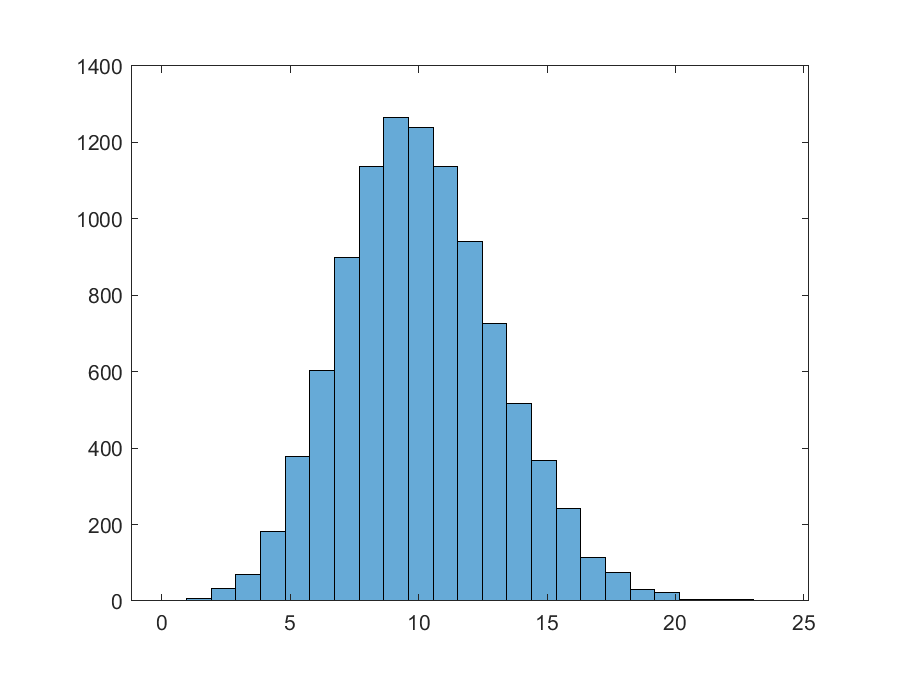
\includegraphics[width=0.75\textwidth]{images/a1_histo.eps}
        
        (b) MLE of $\lambda$ is: 
        $\hat{\mu}_{MLE} = \frac{1}{n} \sum\limits_{k=1}^{n} x_k = 10.0171$

        (c) for $\alpha=1, \beta=1$:
        $$
        \lambda_{MAP} = \frac{\alpha - 1 + \sum_{k=1}^{n} x_k}{n + \beta} = 10.0161
        $$

        (d) for $\alpha=100, \beta=1$:
        $$
        \lambda_{MAP} = \frac{\alpha - 1 + \sum_{k=1}^{n} x_k}{n + \beta} = 10.0260
        $$

        (e) for $\alpha=10, \beta=1$:
        $$
        \lambda_{MAP} = \frac{\alpha - 1 + \sum_{k=1}^{n} x_k}{n + \beta} = 10.0170
        $$

        (f) As number of the data samples is large enough, so I think the approximation in e) is the best which is the closest to the MLE value; 
        The bigger $\alpha$/smaller $\beta$ is, the MAP estimates tend to right-shift from MLE; the smaller $\alpha$/bigger $\beta$ is, the MAP estimates tend to left-shift from MLE.

    \end{solution}
\end{document}